\documentclass[12pt]{report}
\usepackage[top=1in, bottom=1in, left=1in, right=1in, a4paper]{geometry}

 \ifx\pdftexversion\undefined
 \usepackage[dvips]{graphicx}
 \else
 
 \usepackage[pdftex]{graphicx}
 \DeclareGraphicsRule{*}{mps}{*}{}
 \fi
%\usepackage{tabularx,colortbl}
\usepackage{url}
\usepackage{chapterbib}
\usepackage{hyperref}
\usepackage{tabularx}
%\usepackage{tikz}
%\usepackage{pgfplots}
%\usepgfplotslibrary{groupplots} 
%\usepackage{pgf, pgfarrows, pgfnodes}
\usepackage{lscape}
\usepackage{longtable}
\usepackage{float}
\usepackage{url}
\usepackage{multicol}
\usepackage{color}
\usepackage{float}

%\usepackage[none]{hyphenat}
\renewcommand{\bibname}{References}

\setcounter{secnumdepth}{4}
\setcounter{tocdepth}{4}

\begin{document}

\begin{titlepage}
 \begin{center}
\LARGE
\textbf{Cloud based IT Infra with Central Identity} \\
%\vfill
%
\includegraphics[width=3.5cm]{rgukt_logo.jpg}
\vfill
\large
\textbf{\{ Project reboot \}}\\
\vfill
\textbf{Preliminary Project Plan }\\
\vfill
\Large
\underline{\textbf{Project Guide }} \\ 
\large
\underline{} \\
Asst. Prof. Chandra Shaker \\
\normalsize
Dept. of CSE - RGUKT Nuzvid \\
\url{chandra.indra@gmail.com}
\vfill

\Large
\textbf{\underline{ Project Team } } \\
\underline{} \\
\large
\begin{tabular}{l l}
Mr. Aneesh Kumar & \normalsize \url{anush0247@gmail.com} \\
Mr. Nageswarao  & \normalsize \url{anush0247@gmail.com} \\
Mr. Anesh  & \normalsize \url{anush0247@gmail.com} \\
Mr. Jyothi Ram & \normalsize \url{anush0247@gmail.com} 
\end{tabular}

\vfill



\includegraphics[width=3.5cm]{rgukt_logo.jpg} 
\Large
\underline{} \\
\underline{} \\
\normalsize
\textbf{Dept. of Computer Science and Engg. } \\
\textbf{R.G.U.K.T. - Nuzvid } \\
\textbf{Krishna Dt. - Andrha Pradesh - 521202}


\normalsize
\vfill
%\begin{multicols}{2}
%\begin{flushleft}
%\textbf{Start Date} : Sep 2014 \\
%\end{flushleft}
%
%
%\begin{flushright}
%\textbf{End Date} : Jan 2015 \\
%\end{flushright}
%\end{multicols}

\textbf{Sep 2014 -- Jan 2015 }

\end{center}
\end{titlepage}

% \pagebreak \thispagestyle{empty} \textcolor{white}{text} \pagebreak
 
\chapter*{Abstract}
\setcounter{page}{1}
\pagenumbering{roman}
\normalsize
\hspace{0.5cm} The main objective of ``Cloud based IT Infra with Central Identity'' is to develop new IT Infrastracture using private cloud and provide access to all its services using 
Central Identity which can be available to third party developers  as Identity as a service with dynamic role management and resource endpoints. \newline

New private cloud is aimed to develop using opensource tools such as OpenStack, Ubuntu and provide  virtual machines with high computational power and best platform to providing the virtal labs rather than dedicated lab hardware.

%\pagebreak \thispagestyle{empty} \textcolor{white}{text} \pagebreak
%\listoffigures
%\listoftables
\setcounter{page}{2}
\pagenumbering{roman}
\tableofcontents
\pagebreak \thispagestyle{empty} \pagebreak

 
\setcounter{page}{1}
\pagenumbering{arabic}


\chapter{Introduction}

\section{Introduction}
	``Cloud Based IT Infra with Central Identity'' is a complete solution, based on private cloud to enhance and effiecient utilization the IT Infrastructure of an emerging Universities and Organizations with Central Identity for all its users to access its services.\newline

	It is going to developed in 3 phases 
	\begin{itemize}
		\item \textit{Private cloud} 
		\item \textit{Deploying Network Services} 
		\item \textit{Central Identity}
	\end{itemize}
	
\subsection{Private Cloud}

	Private Cloud establishment is targeted for hardware resource pooling, providing high computational and scalable virtual machines for deploying network based applications (smtp, proxy, ftp), web application and Network storage.
	
\subsection{Deploying Network Services}

	Configuration of Uniform hardware experience over the complete university includes single sign on on every device, configuration of mail servers etc.
	
\subsection{Central Identity}

	Essential part that combines normal network services(proxy, mail, etc.) and organizational web \& native applications. In addtion to that this central identity is available to thrid party developers as API with dynamic based role user authentication protocols.	
	

\chapter{Typical Solution}

\section{System under consideration}

	We have observed some organizations are 
	\begin{itemize}
		\item Failed to maintain large user load web services  and network applications.
		\item No Central Identity, Storage \& High capacity hardware resource pool.
		\item Redundent data in each prospect
		\item Inadequate resource requirements for Research.
		\item Dedicated computer course labs like Matlab, VLSI, etc. 
	\end{itemize}

\section{Proposed System}

	To avoid above mentioned observations we are proposing one new system with 
	\begin{itemize}
		\item Cloud based hardware resources clustering.
		\item Central Identity for Network Applicaitons with REST API.
		\item Dynamic user role management.
		\item Providing Virtual Labs (MatLab, etc.,).
		\item High Configurational Virtual Machines for research.
	\end{itemize}

\chapter{Development}

\section{Development Stack}
\begin{figure}[H]
 \centering
 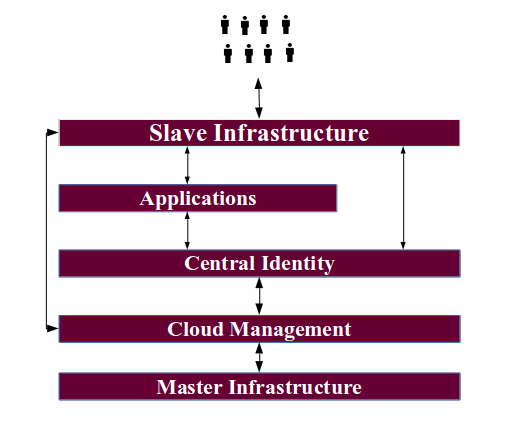
\includegraphics[width=8cm]{./idea.png}
 \caption{Developemnt Stack\label{fig:Developemnt Stack}}
\end{figure}

\section{Development Architecture}
\begin{figure}[H]
 \centering
 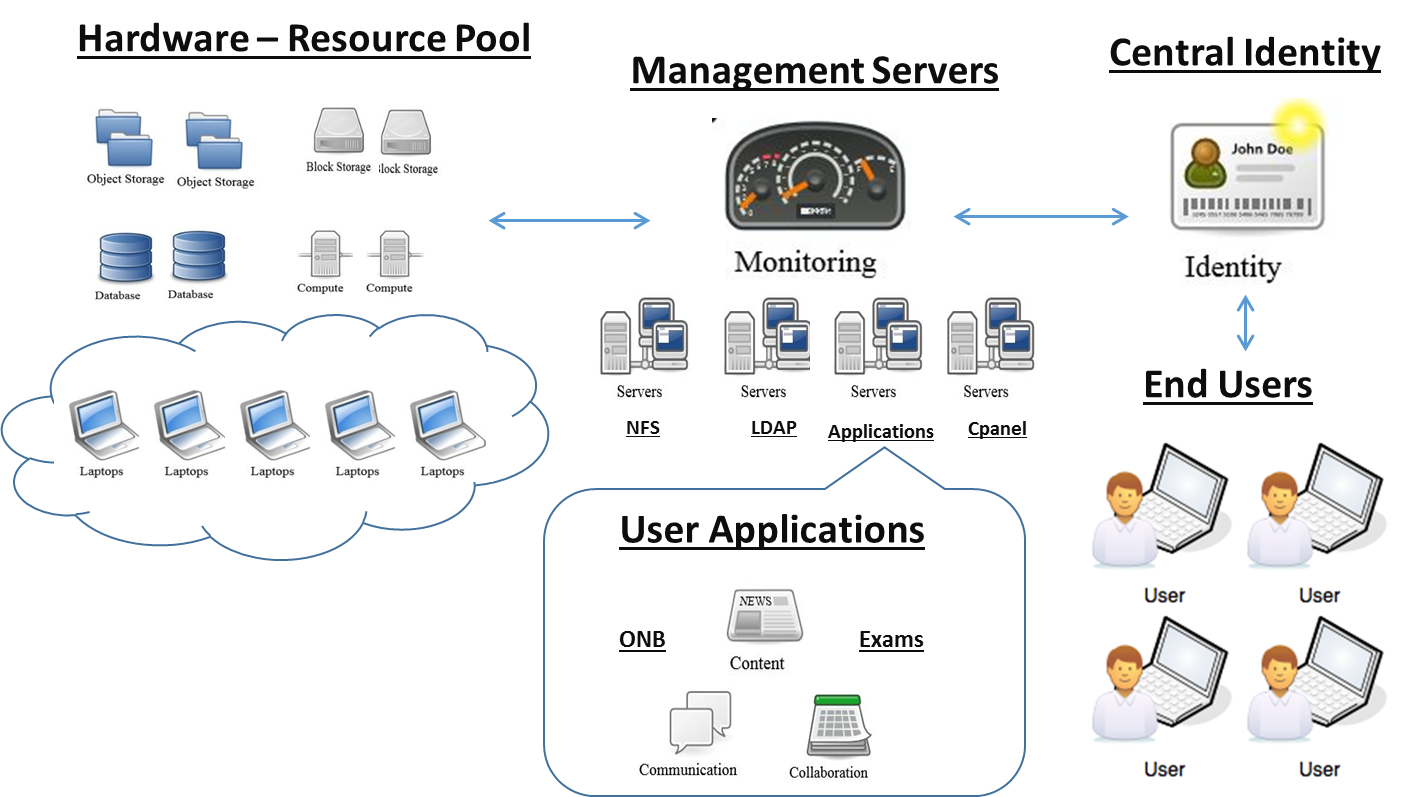
\includegraphics[width=10cm]{./all.png}
 \caption{Archtitecture\label{fig:Archtitecture}}
\end{figure}

\chapter{Design and Approach}

\section{Existing System Specifications}

%	We have been observing that components we are planed develop name private cloud and central identity are already exsisted but key difference here is we want to combine them and extend the central identity as Identity as a service to all emerging developers in that organization with some sort of API calls in  

\begin{itemize}
	\item The environment we observed is our university, it cosists of 7000 students and more than 500+ faculty with 6 core Engineering departments.
	\item Each Department is having strength of 700 students they arrenged these students into various various classes of 60 to 70 each, total 10 to 12 number. 
	\item Each student is provided with one Laptop with 2G RAM, 1.5GHz Clock and 200 GB Harddisk Storage. 
	\item All students are using these sytems for more than 10 hours in a day.
	\item All these students has to provided with course content and course labs, they are maitaining dedicated labs with 50 - 60 machines.
	\item Hence redendent data and failed to moniter the content over those laptops and these labs are useful only at lab hourse most of time they are idle.
\end{itemize}	

\section{Proposed Design and Approach}

	We want to make use of entire departmental hardaware resources more on its students laptops capacity and create a common pool of resources hence easy to maintain and moniter.\\
	
	We want to provide signle sign on implentation in each class of 60-70 laptops. such that user can use his own unique username to access university resources and later he can use the same password for network based or web based applications such as updates, mails, examinations, results etc.\newline
	
	User data can be data is retrevied from the Storage server like nfs while loging in to his laptop in any class room and his laptop's computational and storage capacity is used by the private cloud extentions that it make his laptop as slave node when ever laptop is available.\newline 
	
	User can develop application and they can use Central Identity in their application with user control and access specifations for API calls. \newline
	
\chapter{Implentation and Specifications}

\section{Implentation}

	For maintining above kind of envronment we have to setup one private cloud which will gives the highly scalable virtual machines to server the user need services on fly.\\
	
	We want develop minal system with the above guidelines in a lab environment of 10 Master nodes and 5 client machines with uniform operating system and nfs data share. Later extended upto departmental level.
	
	
\section{Specifications}

	\begin{itemize}
		\item 15 Laptops with below configuration ( 10 Master Nodes + 5 Slave Nodes )
			\begin{itemize}
				\item 4GB RAM, 500 GB Harddisk, Intel i3 processor 1.5GHz Clock
			\end{itemize}
		
		\item Class C Network 
			\begin{itemize}
			 	\item Static IP for Master Nodes
			 	\item DHCP / Static IP for Slave Nodes
			\end{itemize}
			
		\item Uninterrupted power suply for Master Nodes.
		
	\end{itemize}
	
\section{Desired Technologies}

	\begin{itemize}
		\item Opensource private cluod tools such as Openstack, Cloudstack, etc.
		\item Ubuntu 14.04 Server LTS.
		\item LDAP Active Directories, Kerbrose, Squid for Network proxy.
		\item OAuth 2.0 with extended dynamic roles managment.
		\item Nodejs for Implementation of OAuth 2.0 as REST API.
		\item Git for Version control 
		\item Ascii doc / python shpenix \& Latex for Documentation.
	\end{itemize}
	
\section{Expcted Results}

	We are expecting the below results after successfull implemenation of ``Cloud Based IT Infra with Central Identity'' in lab enviroment with above mentioned specifications

	\begin{itemize}	
	\item Hardware resoucre clusters from Master Nodes
	 \begin{itemize}
	 	\item 40 GB RAM
		\item 5TB of Hard disk
		\item 15 GHz Clock Speed	
	 \end{itemize}
		
	\item Hardware resoucre clusters from Slave Node (available only at active period)
	 \begin{itemize}
	 	\item 20 GB RAM
		\item 2TB of Hard disk
		\item 7.5 GHz Clock Speed	
	 \end{itemize}
	 
	\item Well Documented Implementation of Central Identity for 
	 \begin{itemize}
	 	\item Single Sign on of Client Machines.
	 	\item Network applications proxy, mails.
	 	\item University Web Services and Departmental websites.
	 	\item Third party OAuth 2.0 Implemenation as API. 
	 \end{itemize}
	\item Dynamic user role management for both Web and Native applications as API.
	\item Central Cloud Storage Pool.
	\item High Computational Virtual Machines.
	\item Virtual Labs insted of Dedicated labs in Remote Desktop or in SSH protocol.
	\item Content or Data Monitering in a Organization.
	\item Get full recovery and achieve more than 99.99\% services up time.
	\item Extendable to several departments and Universities.
	
	\end{itemize}
	
\pagebreak
\section{Project Time Line}

	Tentative Project Time Line and Deadlines for differnt moudles and break points
	
	\begin{table}[H]
		
		\begin{tabular}{ | l | l | l | l |}
			\hline 
			\textbf{Module} & \textbf{Start Date} & \textbf{End Date} & \textbf{Status} \\
			\hline 
			Central Identiy - Profile, Resourses, Login and & 1st Oct & 8 Oct & \\
			\hline
			Central Identiy - Admin Portal & 8 Oct & 21 Oct & \\
			\hline
			Central Identiy - OAuth API & 8 Oct & 31 Oct & \\
			\hline
			Signle Sign on & 15st Oct & 8 Nov & \\
			\hline
			Private Cloud Construction & 1 Nov & 15 Nov  & \\
			\hline 
			Deploying Applications on Private Cloud & 15 Nov & 8 Dec & \\
			\hline 
			Automation of User deplyment \& Cloud configuration & 21 Nov & 1 Dec & \\
			\hline 
			Integration each Module & 1 Dec & 15 Dec & \\
			\hline
			Unit Testing after Integration & 8 Dec & 21 Dec  & \\
			\hline
			Complete Testing & 21 Dec & 21 Jan &  \\
				
			\hline 
		\end{tabular}
		
	\end{table}
	
	\begin{itemize}
		\item Unit Testing of each module for 2 -- 3 days.
		\item Each module has to docuemnted in parallel.
	\end{itemize}
	
\chapter{References}

\section{Web References}

\begin{itemize}
\item Ubnutu OS, http://www.ubuntu.com/
\item Openstack, https://openstack.org/
\item OAuth 2.0, http://oauth.net/
\item Node.js https://nodejs.org
\item Git, https://github.com
\item Ascii doc, http://asciidoc.org
\item Bootstrap, http://getbootstrap.com 
\item Stack Overflow http://stackoverflow.com/

\end{itemize}
		

\end{document}